\chapter{Конструкторская часть}

Ниже приведены схемы алгоритмов, упомянутых в аналитической части:
\begin{itemize}
	\item на рисунке~\ref{fig:std_scheme} --- схема стандартного алгоритма умножения матриц;
	\item на рисунке~\ref{fig:strassen_scheme} --- схема алгоритма Штрассена;
	\item 
\end{itemize}
\begin{figure}[H]
	\centering
	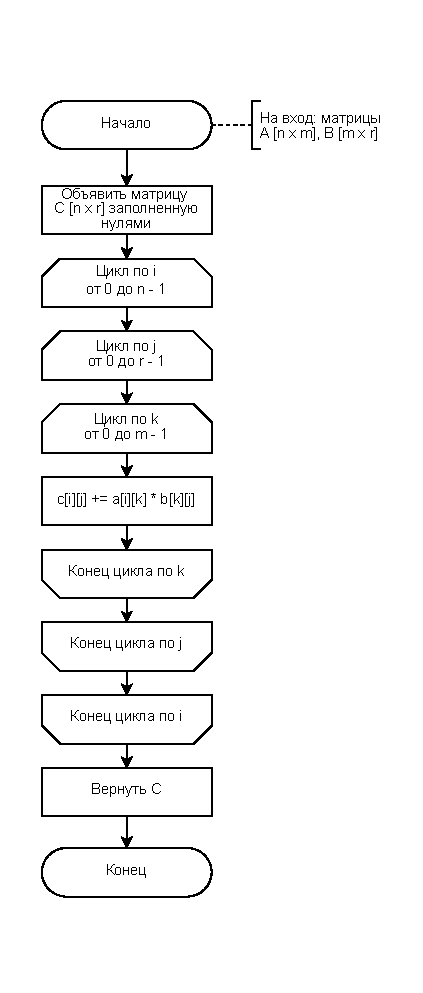
\includegraphics[width=0.8\textwidth]{std_scheme.pdf}
	\caption{Схема алгоритма линейного поиска}
	\label{fig:std_scheme}
\end{figure}
\begin{figure}[H]
	\centering
	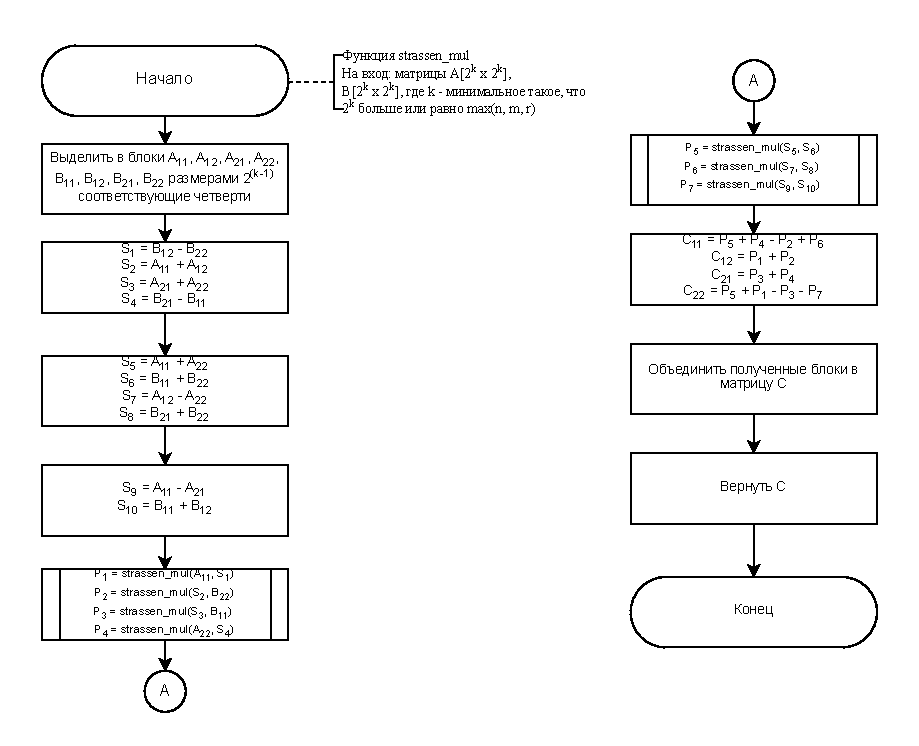
\includegraphics[width=0.8\textwidth]{strassen_scheme.pdf}
	\caption{Схема алгоритма Штрассена}
	\label{fig:strassen_scheme}
\end{figure}
\section{Требования к реализации алгоритмов}

Реализации алгоритмов должны удовлетворять следующим общим требованиям:
\begin{itemize}[label=---]
	\item входные данные: массив целых чисел, элемент для поиска, представленный целым числом;
	\item выходные данные: индекс вхождения элемента или -1, если элемент не найден.
\end{itemize}

К алгоритму бинарного поиска предъявляется дополнительное требование: входной массив должен быть упорядочен по неубыванию.
\section*{Вывод}

На основе аналитической части построены схемы алгоритмов для реализации.

\clearpage